%!TEX root = main.tex

\chapter{Modulation}
\label{chap:modulation}


\begin{figure}[H]
	\begin{center}
		\includegraphics[width = 14cm]{img/surface-modulation_3.jpg}
		\caption{``Surface Modulation'' by Richard Sweeney}
		\label{fig:Surface Modulation}
	\end{center}
\end{figure}


\begin{center}
\begin{figure}[h!]
\tikzset{concept/.append style={fill={none}}}
\begin{tikzpicture}
  \path[mindmap,concept color=black,text=black]
    node[concept] {Modulation}
    [clockwise from=0]
    child[concept color=red!50!black] {
      node[concept] {AM}
      % }
      [clockwise from=90]
      child { node[concept] {Envelopes} }
      child { node[concept] {AM} }
      child { node[concept] {Ring Modulation} }
      % child { node[concept] {pro\-gramming languages} }
      % child { node[concept] {software engineer\-ing} }
    }
    child[concept color=blue] {
      node[concept] (fm) {FM}
      [clockwise from=-30]
    }
    child[concept color=red] { node[concept] (pm){Phase Modulation} }
    child[concept color=orange] { node[concept] (sd) {Sound design Challenge} }
    child[concept color=green] { node[concept] (conv) {Convolution} };


\begin{pgfonlayer}{background}
    \draw [circle connection bar]
      (fm) edge (sd)
      (fm) edge (pm);
  \end{pgfonlayer}

\end{tikzpicture}
\caption{Lecture Contents}
\end{figure}
\end{center}


% \section{Notizen}

% kürzer. Modulation als sub einheit einplanen.
% Sounddesign challg. halbe stunde ok..

% Passt garnicht: (weil eher additive synth)
% https://www.youtube.com/watch?v=oKv9S6mxnXE

% Convolution anreissen?
% Notation durchgehen.

% Aliasing besprochen?
% \href{https://www.youtube.com/watch?v=GBtHeR-hY9Y}{Water experiment}
% (youtube \glqq{}The Secret to Levitation\grqq{})

% AM, tremolo

% Envelopes in pd

% FM, vibrato

% sounddesign chall.

% Hü

\section{Convolution}
\label{sub:conv}
Before talking about modulation, we should quickly look at what's convolution\footnote{'Faltung' in German}.\\
Convolution is a mathematical operation, widely used in signal processing but also in other fields. Convolution of two functions, say, $x$ and $h$ is typically denoted as $x*h$. \textbf{Note that $*$ does not mean multiplication here, it means convolving $x$ with $h$}. Obviously this can lead to confusion in some cases, but notation problems are not uncommon in sciences.\footnote{e.g while mathematicians use $i$ as the imaginary number, electrical engineering folks use $j$ (their $i$ is electrical current.).}\\

We will define Convolution of a function $x$ with a convolution kernel $h$ of length $N$as\footnote{You will find different definitions online. The given definition seems more intuitive but is not very common. Here is a common one:$y(n) = \sum_{k=-\infty}^{\infty} x(k) h (n-k)$}:

\begin{equation}
y(n) = \sum_{k=0}^{N-1} x(n-k) h (k)
\end{equation}
In words: for every output sample $y(n)$ take the current input sample $x(n)$ times the first sample of the convolution Kernel $h(0)$ plus take the previous input sample $x(n-1)$ times the second sample of the convolution kernel $h(1)$ plus the third last input sample $x(n-2)$ times the third sample of the convolution kernel $h(2)$ and so on... until the $Nth$ sample of $h$. It can be viewed as a a weighted average of the previous input samples, with weighting coefficients found in $h$.

We will look at convolution in a later chapter. If you  are eager to know more about convolution can have a look at
\href{https://youtu.be/_vyke3vF4Nk?t=25m14s}{this}\footnote{https://youtu.be/\_vyke3vF4Nk?t=25m14s}. \link{http://www.songho.ca/dsp/convolution/convolution2d\_example.html}{Here} is an example of convolution in 2D. Convolution in 2D is actually a bit easier to understand and is usually done to achieve a blur effect on an image or video. But why mention convolution if it is not explained at this point? Amplitude modulation and convolution just have a very close relationship, an that is:
\important{Multiplying two signals in the time domain is equivalent to convolution in the frequency domain and convolution in the time domain is equivalent to multiplication in the frequency domain.
}



\section{AM} % (fold)
\label{sub:AM}
In this section we will try amplitude modulation. Amplitude modulation is used for radio communication (so you'll need to understand this as a technician, modulation techniques are extremely important and this is maybe the simplest one) but also in sound design. We will try to understand the problem from different perspectives at once:
\begin{itemize}
	\item Doing some math
	\item listening to it
	\item brining it in context to beating waves
	\item seeing it as convolution in the frequency domain
\end{itemize}

Amplitude modulation means modulating the amplitude of a signal(surprise!). Modulating means changing over time by another signal. So we have some signal, say, a sine wave, and change its amplitude with another signal, say, another sine wave. Taking this concept and reducing it radically, we end up with figure \ref{fig:simpleAM}.

\begin{figure}[H]
	\begin{center}
		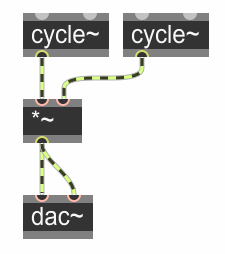
\includegraphics{img/ringNaive.png}
		\caption{Simplest form of ``Ring modulation''.}
		\label{fig:simpleAM}
	\end{center}
\end{figure}
Of course, we get no sound in figure \ref{fig:simpleAM} because the frequencies are not initialized, but it shows the general principle. The caption of that figure says ``Ring Modulation''. Let's quickly get some vocabulary straight:\\
\begin{itemize}
	\item ``Amplitude modulation'' might mean any modulation of amplitude
	\item ``Ring Modulation'' means \textit{bi-polar} amplitude modulation.
	\item In sound design, ``Amplitude Modulation'' might specifically mean unipolar amplitude modulation.
\end{itemize}

And some more vocabulary to put what we are doing in a musical context:
\begin{itemize}
	\item Modulating the amplitude is called ``Tremolo'' in music \footnote{sadly, the fender Stratocaster's ``Tremolo Arm'' is used to control the pitch. Ignore Fender, they got it wrong. You can trust that most guitar players are confused because of this.}
	\item Modulating the pitch or frequency (``FM'') is called ``vibrato'' in a musical context.\footnote{Maybe think about it like this: The F in FM is a bit like the v in vibrato. Just to avoid confusion..}
\end{itemize}

Enough words, let's look at what AM looks like, look at figure \ref{fig:AMViz}.

\begin{figure}[h!]
	\centering
	\includegraphics[width=\textwidth]{AMviz.png}
	\caption[AM time domain]
	{Looking at AM in the time domain}
	\label{fig:AMViz}
\end{figure}

\begin{question}
	If we would listen to the signal depicted in the bottom plot of figure \ref{fig:AMViz}, what do you think we would hear? Try to imagine! If you can't, use pure data to test it! That's why we are using pd.
\end{question}
\begin{Answer}
	We would hear a 30Hz sine wave repeatedly rising and falling in amplitude.
\end{Answer}

\begin{question}
	Next question, same plot, same signal. So hopefully you found out that we hear a 30 Hz sine with rising and falling amplitude. At what frequency does the amplitude rise and fall? Remember we are modulating with a 1 Hz sine.
\end{question}
\begin{Answer}
	Two Hertz.
\end{Answer}

You can try out plotting what happens with different frequency settings in \link{https://colab.research.google.com/drive/1oO3ApcIfvcUoIqv9\_nDS-HNl8B4Gf5hl}{this Notebook}.

Maybe you remember from the waveshaping chapter that we actually calculated what frequencies should come out of AM. Also maybe you remember that:

\important{
Amplitude Modulation produces sum and difference frequencies of the input frequencies.
\begin{equation}
	cos(a)\cdot cos(b) = \frac{cos(a+b) + cos(a-b)}{2}
\end{equation}
}
But here we still hear the 30 Hz, just getting louder and softer, so what's wrong?\\
So, let's calculate this. We have two oscillators, $x_1(t) = cos(30t2\pi)$ and $x_2(t)=cos(t2\pi)$. We multiply them, ending up with:

\begin{equation}
	y(t) = cos(30t2\pi) \cdot cos(t2\pi)
\end{equation}
Ok, the above formula tells us this means:
\begin{equation}
	y(t) = \frac{cos(30t2\pi+t2\pi)+cos(30t2\pi-t2\pi)}{2}
\end{equation}
We can now simplify to:
\begin{equation}
	y(t) = \frac{cos((30+1)t2\pi)+cos((30-1)t2\pi)}{2} = \frac{cos(31t2\pi)+cos(29t2\pi)}{2}
\end{equation}

Hm, so we get out a 31Hz and 29Hz oscillator. What about that rising and falling in amplitude that we hear \textit{and} observe in the plot, surely there must be something wrong! Do you have a solution to this?\\

Let's use pure data to help us understand. Make two oscillators, one with 29Hz and one with 31Hz, what do you hear?

\begin{figure}[h!]
	\centering
	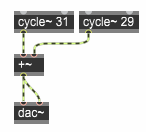
\includegraphics{beating.png}
	\caption[adding two oscillators]
	{Adding two oscillators with frequencies very close to each other}
	\label{fig:beating}
\end{figure}

If you listen to what is depicted in figure \ref{fig:beating}, you will in fact hear the same as if you do the 30Hz /1 Hz amplitude modulation (which indicates that our formula above is correct). What we hear is a phenomenon called beating(``Schwebung''). The phase of the two oscillators is canceling each other out at regular intervals because the frequencies are so close to each other. In fact the frequency of the beating $f_{beat}$ is always
\begin{equation}
	f{beat}=|f_1-f_2|
\end{equation}
So the difference of the two frequencies.


% \comm{vline and envelop description missing}
% \begin{figure}[H]
% 	\begin{center}
% 		\includegraphics[width = 14cm]{img/simpleEnv.png}
% 		\caption{caption}
% 		\label{fig:name}
% 	\end{center}
% \end{figure}

\section{FM} % (fold)
\label{sub:FM}

Frequency modulation can be used to modulate the frequency, meaning to vary the pitch of a sound, see figure \ref{fig:fmSlow}. But it can also be used to generate overtones and an overall richer spectrum, see figure \ref{fig:fmFast}. The two ``different versions'' only differ from each other by different parameter\footnote{We see which parameters can be adjusted in a minute. But if you want to know them now: modulation frequency, modulation amount and carrier frequency.} values being used.
We can think of Frequency Modulation (FM) as something of the form:

\begin{equation}
	y(t) = cos(cos(b))
\end{equation}

This really is a simplification, but the overall structure of the formula is correct.
% FM is mathematically very similar to phase modulation.
Looking at figure \ref{fig:fmIdea} we can see the very basic idea implemented in pure data.
\begin{figure}[H]
	\begin{center}
		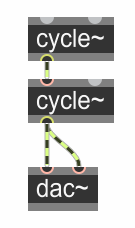
\includegraphics{img/FMgeneral.png}
		\caption{The General Idea of FM}
		\label{fig:fmIdea}
	\end{center}
\end{figure}

Since the frequencies of the oscillators are not set, we won't hear anything when building this patcher. But looking at it may reveal that the idea simply is to control the frequency of an oscillator using another oscillator.\\
We can expand the patcher by adding some math to make it more usable, as in figure \ref{fig:fmNaive}.

Naive parameters are ${f_c}$ (Carrier Frequency), ${f_m}$ (Modulator Frequency), and ${A_m}$ (modulation Amount).

\begin{figure}[H]
	\begin{center}
		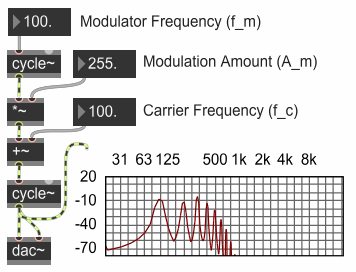
\includegraphics{img/FMnaive.png}
		\caption{Naive Implementation with Direct Parametrization.}
		\label{fig:fmNaive}
	\end{center}
\end{figure}

\important{

The output frequencies will be
\begin{equation}
	f_c \pm n \cdot f_m
\end{equation}

for $n$ being all integers. So the carrier frequency plus and minus integer multiples of the modulation frequency. We get many (theoretically infinitely) many overtones with different amplitudes this way.
}
\bgInfo{
	The amplitudes of the different frequencies are determined by Bessel functions which makes it so seemingly random.
		\centering
		\includegraphics[width=11cm]{bessel}
}


Typically, FM is controlled via \textit{Index}, \textit{Ratio}, and fundamental Frequency.
The Index, ${I}$ is given by Modulation Depth and Modulator Frequency.


% =============Something is wrong with this.============================

% \begin{mdframed}[backgroundcolor=black!10,rightline=false,leftline=false]
\bgInfo{
\begin{equation}
I = \frac{A_m}{f_m} % verified via http://computermusicresource.com/FM.synthesis.html
\end{equation}

A more controllable Implementation will generate the naive parameters from a Ratio, ${R}$, the Carrier Frequency and the Index:
\begin{equation}
	f_m = \frac{f_c}{R}
\end{equation}

\begin{equation}
	A_m = I \cdot f_m
\end{equation}

\begin{figure}[H]
	\begin{center}
		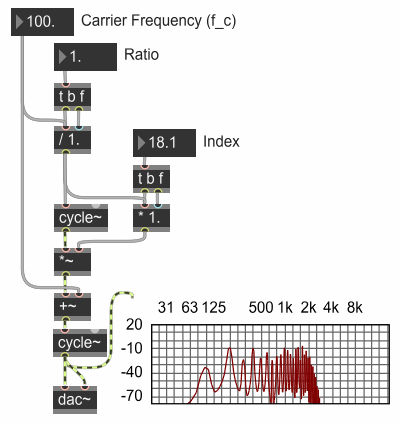
\includegraphics{img/FMcorrect.png}
		\caption{FM with Index and Ratio}
		\label{fig:fmComplete}
	\end{center}
\end{figure}

But there are also different implementations such as:
\begin{figure}[H]
	\centering
	\includegraphics[width=5cm]{fmMillerPuckette}
	\caption[miller Puckette FM]
	{Fm implementation from \cite{miller_puckette_theory_2006}}
	\label{fig:label}
\end{figure}

% ===========FIND EN EXPLANATION FOR THE ABOVE FM implementations=============


% \end{mdframed}
% =========================================================================
}

\begin{figure}[h!]
	\centering
	\includegraphics[width=\textwidth]{FMslow}
	\caption[FM visualization, low freq]
	{Modulator frequency: 1Hz, Crarrier Frequency 50 Hz, Modulation Amount 10. Please ignore the labeling of the Y axis of the spectrum plot($10^0$). It is wrong. The y axis goes from 0 to nyquist=22050Hz.}
	\label{fig:fmSlow}
\end{figure}


\begin{figure}[H]
	\centering
	\includegraphics[width=\textwidth]{FMfast}
	\caption[FM visualization, hi freq]
	{Modulator frequency: 100Hz, Crarrier Frequency 1000 Hz, Modulation Amount 0.5. Please ignore the labeling of the Y axis of the spectrum plot($10^0$). It is wrong. The y axis goes from 0 to nyquist=22050Hz.}
	\label{fig:fmFast}
\end{figure}


\section{Key Points}
\begin{itemize}
	\item Make sure you understand the differences between AM and FM
	\item Make sure you recognize what form of modulation is present if you see a patcher or a simplfied formula (like: $sin(a) \cdot sin(b)$ what form of modulation is this?)
	\item make sure you could make such a simplified formula if you see a patch and vice versa.
	\item make sure you know what frequencies result from an amplitude modulation
	\item make sure you know what frequencies result from a frequency modulation
\end{itemize}

% \section{Hausübung}
% \label{sub:Hausuebung}
% Andy Farnell, \href{http://aspress.co.uk/ds/pdf/pd_intro.pdf}{pd intro} chapter 6, lesen
